%!TEX program = xelatex
\documentclass[times,namecite]{goose-article}

\usepackage{lipsum,verbatim,mdframed,pdflscape,array}
\usepackage{arydshln}

\usepackage[utf8]{inputenc}

% Default fixed font does not support bold face
\DeclareFixedFont{\ttb}{T1}{txtt}{bx}{n}{12} % for bold
\DeclareFixedFont{\ttm}{T1}{txtt}{m}{n}{12}  % for normal

% Custom colors
\usepackage{color}
\definecolor{deepblue}{rgb}{0,0,0.5}
\definecolor{deepred}{rgb}{0.6,0,0}
\definecolor{deepgreen}{rgb}{0,0.5,0}

\usepackage{listings}

% Python style for highlighting
\newcommand\pythonstyle{\lstset{
language=Python,
basicstyle=\ttm,
otherkeywords={self},             % Add keywords here
keywordstyle=\ttb\color{deepblue},
emph={MyClass,__init__},          % Custom highlighting
emphstyle=\ttb\color{deepred},    % Custom highlighting style
stringstyle=\color{deepgreen},
frame=tb,                         % Any extra options here
showstringspaces=false            %
}}

% Python environment
\lstnewenvironment{python}[1][]
{
\pythonstyle
\lstset{#1}
}
{}

\newcolumntype{L}[1]{>{\raggedright\let\newline\\\arraybackslash\hspace{0pt}}m{#1}}
\newcolumntype{C}[1]{>{\centering\let\newline\\\arraybackslash\hspace{0pt}}m{#1}}
\newcolumntype{R}[1]{>{\raggedleft\let\newline\\\arraybackslash\hspace{0pt}}m{#1}}

\newcommand{\Grad}{\vec{\nabla}}

\title{%
  Periodicity
}

\author{T.W.J.~de~Geus$^{*,}$}

\contact{%
  $^*$Contact: %
  \href{mailto:tom@geus.me}{tom@geus.me} %
  \hspace{1mm}--\hspace{1mm} %
  \href{http://www.geus.me}{www.geus.me}%
}

\hypersetup{pdfauthor={T.W.J. de Geus}}

\header{}

\begin{document}

\maketitle

This document is aimed at explaining different available strategies to perform finite element computations on a periodic domain. To make our life a little simpler, this document is based on a two-dimensional problem where the unknowns at the nodes, $u$, are scalars. In this setting one can think of Poisson's equation
\begin{equation}
  \bigtriangleup u ( \vec{x} ) = q ( \vec{x} ) \qquad \forall \; \vec{x} \in \Omega
\end{equation}

Using the finite element strategy of solving this in a weak form and an discretization using finite elements, one ends up with the following nodal equilibrium equations
\begin{equation}
  \underline{f} ( \underline{u} ) = \underline{q}
\end{equation}
This equation is then usually linearized to obtain
\begin{equation} \label{eq:system}
  \underline{\underline{A}}_{(i)} \, \delta \underline{u}
  =
  \underline{q}_{(i)} - \underline{f}_{(i)}
  =
  \underline{b}_{(i)}
\end{equation}

For the simple finite element mesh shown in Figure~\ref{fig:mesh}(b), the system matrix, $\underline{\underline{A}}$, and the right-hand-side, $\underline{b}$, are specified in Appendix~\ref{sec:system}. The notation follows the typical assembly procedure of a finite element code (see Appendix~\ref{sec:code}), whereby the contributions of the different element matrices/vectors are included as $\left( . \right)^\mathrm{(element\, number)}_\mathrm{local\, node\, number(s)}$. Note that the definition of the local element numbers for this mesh are shown in Figure~\ref{fig:mesh}(a).

In assuming periodicity, $u$ is decomposed in a global contribution $\bar{u}$, plus a fluctuation $u^\star$:
\begin{equation}
  u = \bar{u} + u^\star
\end{equation}
The global contribution is some finite affine field for which
\begin{equation}
  \int_\Omega \, \Grad u^\star \;\mathrm{d}\Omega = \vec{\bm{F}}
\end{equation}
while for the periodic fluctuations
\begin{equation}
  \int_\Omega \, \Grad u^\star \;\mathrm{d}\Omega = 0
\end{equation}

\begin{figure}[htp]
  \centering
  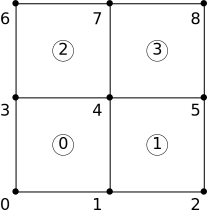
\includegraphics[width=.8\textwidth]{mesh}
  \caption{Finite element used to exemplify the linear system: (a) the local node numbering inside each element, (b) the mesh including \textit{\textsf{element}} and (global) node numbers, and (c) the mesh including periodic repetitions complete with the \textit{\textsf{element}} numbers, the (global) node numbers of the independent nodes that remain, and all periodic repetitions.}
  \label{fig:mesh}
\end{figure}

For this example, assuming periodicity implies in assuming the nodes on the right side of the mesh are the periodic repetitions of those on the left side, and likewise for the nodes on the top and bottom; whereby one side is shifted by the global affine field compared to the other. Let us ignore the latter for a moment, and just focus on the periodic fluctuations. In that case
\begin{equation}
\begin{aligned}
  u^\star_{ 4} &= u^\star_{ 1} \\
  u^\star_{13} &= u^\star_{ 1} \\
  u^\star_{16} &= u^\star_{ 1} \\
  u^\star_{ 8} &= u^\star_{ 5} \\
  u^\star_{18} &= u^\star_{ 9} \\
  u^\star_{14} &= u^\star_{ 2} \\
  u^\star_{15} &= u^\star_{ 3}
  \label{eq:tyings}
\end{aligned}
\end{equation}
We will start by dividing the system in independent, $i$, and dependent, $d$, degrees-of-freedom (DOFs). By this it is meant that the dependent DOFs are periodic repetitions, while independent DOFs are all the remaining ones. For the mesh from Fig.~\ref{fig:mesh}(b):
\begin{align}
  i &= \big[ 1, 2, 3, 5, 6, 7, 9, 10, 11 \big] \\
  d &= \big[ 4, 8, 12, 13, 14, 15, 16 \big]
\end{align}
We continue by renumbering the DOFs such that
\begin{align}
  i &= 1 .. 9 \\
  d &= 10 .. 16
\end{align}
as is shown in Fig.~\ref{fig:mesh}(c). The programmatic consequences can be found in Appendix~\ref{sec:code:per}. Once we have done this we can write Eq.~\eqref{eq:tyings} as a matrix equation
\begin{equation}
  \underline{u}^\star_{d} = \underline{\underline{C}}_\mathrm{di} \underline{u}^\star_{i}
\end{equation}
with
\begin{equation}
  \underline{\underline{C}}_\mathrm{di} =
  \left[
  \begin{array}{ccccccccc}
    1 & 0 & 0 & 0 & 0 & 0 & 0 & 0 & 0 \\
    0 & 0 & 0 & 1 & 0 & 0 & 0 & 0 & 0 \\
    0 & 0 & 0 & 0 & 0 & 0 & 1 & 0 & 0 \\
    1 & 0 & 0 & 0 & 0 & 0 & 0 & 0 & 0 \\
    0 & 1 & 0 & 0 & 0 & 0 & 0 & 0 & 0 \\
    0 & 0 & 1 & 0 & 0 & 0 & 0 & 0 & 0 \\
    1 & 0 & 0 & 0 & 0 & 0 & 0 & 0 & 0 \\
  \end{array}
  \right]
\end{equation}
We can use this to eliminate the dependent DOFs from the system of Eq.~\ref{eq:system}. First we partition the system in independent and dependent DOFs
\begin{equation}
  \begingroup
  \renewcommand*{\arraystretch}{1.5}
  \begin{bmatrix}
  \underline{\underline{A}}^{(i)}_{ii} & \underline{\underline{A}}^{(i)}_{id} \\
  \underline{\underline{A}}^{(i)}_{di} & \underline{\underline{A}}^{(i)}_{dd}
  \end{bmatrix}
  \,
  \begin{bmatrix}
  \delta \underline{u}_{i} \\
  \delta \underline{u}_{d}
  \end{bmatrix}
  =
  \begin{bmatrix}
  \underline{b}^{(i)}_{i} \\
  \underline{b}^{(i)}_{d}
  \end{bmatrix}
  \endgroup
\end{equation}
and then apply the node dependency:
\begin{equation}
  \left[
  \underline{\underline{A}}^{(i)}_{ii}
  +
  \underline{\underline{C}}_{di}^\mathsf{T}
  \underline{\underline{A}}^{(i)}_{di}
  +
  \underline{\underline{C}}_{di}^\mathsf{T}
  \underline{\underline{A}}^{(i)}_{dd}
  \underline{\underline{C}}_{di}
  \right]
  \,
  \delta \underline{u}^\star_{i}
  =
  \left[
  \underline{b}^{(i)}_{i}
  +
  \underline{\underline{C}}_{di}^\mathsf{T}
  \underline{b}^{(i)}_{d}
  \right]
\end{equation}
Starting from the original system in Appendix~\ref{sec:system}, this system is detailed in Appendix~\ref{sec:system:static-condensation}.

Once this system has been solved, the dependent DOFs can be reconstructed as follows
\begin{equation}
  \delta \underline{u}^\star_{d}
  =
  \underline{\underline{C}}_{di}
  \delta \underline{u}^\star_{i}
\end{equation}

From an implementation perspective this can be done much simpler by computing the element arrays as usual, but directly assembling to the independent DOFs only. In this case the dependent DOFs get the number of their periodic counterpart, see Appendix~\ref{sec:code:per:assembly}. The resulting system is included in Appendix~\ref{sec:system:periodic-assembly}, which is indeed exactly the same as in Appendix~\ref{sec:system:static-condensation}.

The only question which remains is to introduce $\bar{u}$ to the system. We can do this before the first iteration:
\begin{equation}
  \underline{u}_{(0)} = \underline{\bar{u}}
\end{equation}
The iterative update will not change the mean, hence
\begin{equation}
  \underline{u}
  =
  \underline{\bar{u}}
  +
  \delta \underline{u}^\star_{(0)}
  +
  \delta \underline{u}^\star_{(1)}
  +
  \delta \underline{u}^\star_{(2)}
  +
  \ldots
\end{equation}
One way to construct $\underline{\bar{u}}$ is as follows
\begin{equation}
  \underline{u} = \vec{\bm{F}} \cdot ( \underline{\vec{X}} - \vec{X}_\mathrm{ref} )
\end{equation}
whereby we take node $1$ as reference.

The final thing we can to is to realize that there is an antagonist of $\vec{\bm{F}}$, namely $\vec{\bm{B}}$, which we can now compute for post-processing, but not control. Should we want to, we have to introduce extra degrees of freedom for $\vec{\bm{F}}$ (in this case the number of extra DOFs is equal to the number of dimensions). These DOFs can be used to apply mixed conditions on $\vec{\bm{F}}$ and $\vec{\bm{B}}$.

We will perform the implied volume averaging using a boundary integral. Ultimately this results in the following tying relations
\begin{equation}
\begin{aligned}
  u_{ 4} &= u_{ 1} \hspace*{2mm} + \hspace*{2mm} \vec{\bm{F}} \cdot \big( \vec{X}_{ 4} \hspace*{-3mm}&- \vec{X}_{ 1} \big)  \\
  u_{13} &= u_{ 1} \hspace*{2mm} + \hspace*{2mm} \vec{\bm{F}} \cdot \big( \vec{X}_{13} \hspace*{-3mm}&- \vec{X}_{ 1} \big)  \\
  u_{16} &= u_{ 1} \hspace*{2mm} + \hspace*{2mm} \vec{\bm{F}} \cdot \big( \vec{X}_{16} \hspace*{-3mm}&- \vec{X}_{ 1} \big)  \\
  u_{ 8} &= u_{ 5} \hspace*{2mm} + \hspace*{2mm} \vec{\bm{F}} \cdot \big( \vec{X}_{ 8} \hspace*{-3mm}&- \vec{X}_{ 5} \big)  \\
  u_{18} &= u_{ 9} \hspace*{2mm} + \hspace*{2mm} \vec{\bm{F}} \cdot \big( \vec{X}_{18} \hspace*{-3mm}&- \vec{X}_{ 9} \big)  \\
  u_{14} &= u_{ 2} \hspace*{2mm} + \hspace*{2mm} \vec{\bm{F}} \cdot \big( \vec{X}_{14} \hspace*{-3mm}&- \vec{X}_{ 2} \big)  \\
  u_{15} &= u_{ 3} \hspace*{2mm} + \hspace*{2mm} \vec{\bm{F}} \cdot \big( \vec{X}_{15} \hspace*{-3mm}&- \vec{X}_{ 3} \big)
  \label{eq:tyings:global}
\end{aligned}
\end{equation}
whereby each component of $\vec{\bm{F}}$ is one of the extra, \emph{virtual}, DOFs. After renumbering, we have the following tying relations
\begin{equation}
  \underline{u}_{d} = \underline{\underline{C}}_\mathrm{di} \underline{u}_{i}
\end{equation}
with
\begin{equation}
  \underline{\underline{C}}_\mathrm{di} =
  \left[
  \begin{array}{ccccccccc:cc}
    1 & 0 & 0 & 0 & 0 & 0 & 0 & 0 & 0 & L_x &   0 \\
    0 & 0 & 0 & 1 & 0 & 0 & 0 & 0 & 0 & L_x &   0 \\
    0 & 0 & 0 & 0 & 0 & 0 & 1 & 0 & 0 & L_x &   0 \\
    1 & 0 & 0 & 0 & 0 & 0 & 0 & 0 & 0 &   0 & L_y \\
    0 & 1 & 0 & 0 & 0 & 0 & 0 & 0 & 0 &   0 & L_y \\
    0 & 0 & 1 & 0 & 0 & 0 & 0 & 0 & 0 &   0 & L_y \\
    1 & 0 & 0 & 0 & 0 & 0 & 0 & 0 & 0 & L_x & L_y \\
  \end{array}
  \right]
\end{equation}
where $L_x$ and $L_y$ are the dimensions of the cell in Fig.~\ref{fig:mesh}(b,c). Starting from the original system extended with the extra DOFs, in Appendix~\ref{sec:system:sec:system:static-condensation-virtual}, the final system is given in Appendix~\ref{sec:system:sec:system:static-condensation-virtual:reduced}. Compared to the system in Appendix~\ref{sec:system:static-condensation} one observes that the systems that belong the normal DOFs are identical, while the extra DOFs are clearly tied to the mean.

\appendix

\newpage
\section{Finite element mesh from Figure~\ref{fig:mesh} -- basic program structure -- non-periodic}
\label{sec:code}

\begin{python}
ndim = 2

x = [
  [ 0.    , 0.    ],
  [ 1./3. , 0.    ],
  [ 2./3. , 0.    ],
  [ 1.    , 0.    ],
  [ 0.    , 1./3. ],
  [ 1./3. , 1./3. ],
  [ 2./3. , 1./3. ],
  [ 1.    , 1./3. ],
  [ 0.    , 2./3. ],
  [ 1./3. , 2./3. ],
  [ 2./3. , 2./3. ],
  [ 1.    , 2./3. ],
  [ 0.    , 1.    ],
  [ 1./3. , 1.    ],
  [ 2./3. , 1.    ],
  [ 1.    , 1.    ],
]

u = zeros( ( coor.shape ) )

connectivity = [
  [ 0,  1,  5,  4],
  [ 1,  2,  6,  5],
  [ 2,  3,  7,  6],
  [ 4,  5,  9,  8],
  [ 5,  6, 10,  9],
  [ 6,  7, 11, 10],
  [ 8,  9, 13, 12],
  [ 9, 10, 14, 13],
  [10, 11, 15, 14],
]

for ielem,elem in enumerate(connectivity):

  for idim in range(ndim):
    xe[:,idim] = x[elem,idim]

  ...

  for i,idof in enumerate(elem):
    for j,jdof in enumerate(elem):
      A[idof,jdof] += Ael[i,j]

  for i,idof in enumerate(elem):
    b[idof] += bel[i]
\end{python}

\newpage
\section{Finite element mesh from Figure~\ref{fig:mesh} -- basic program structure -- periodic}
\label{sec:code:per}

\begin{python}
...

nni  = 9
nnd  = 7
dofs = [ 0, 1, 2, 9, 3, 4, 5, 10, 6, 7, 8, 11, 12, 13, 14, 15 ]

for ielem,elem in enumerate(connectivity):

  for idim in range(ndim):
    xe[:,idim] = x[elem,idim]

  ...

  for i,inode in enumerate(elem):
    for j,jnode in enumerate(elem):
      A[ dofs[inode], dofs[jnode] ] += Ael[i,j]

  for i,inode in enumerate(elem):
    b[ dofs[inode] ] += bel[i]

A_ii = A[:nni,:nni]
...

b_i = b[:nni]
...
\end{python}

\newpage
\section{Finite element mesh from Figure~\ref{fig:mesh} -- basic program structure -- periodic}
\label{sec:code:per:assembly}

\begin{python}
...

nni  = 9
nnd  = 7
dofs = [ 0, 1, 2, 0, 3, 4, 5, 3, 6, 7, 8, 6, 0, 1, 2, 0 ]

for ielem,elem in enumerate(connectivity):

  for idim in range(ndim):
    xe[:,idim] = x[elem,idim]

  ...

  for i,inode in enumerate(elem):
    for j,jnode in enumerate(elem):
      A_ii[ dofs[inode], dofs[jnode] ] += Ael[i,j]

  for i,inode in enumerate(elem):
    b_i[ dofs[inode] ] += bel[i]

...
\end{python}

\pagestyle{empty}
\setlength\parindent{0pt}
\newgeometry{landscape,left=40mm,bottom=5mm,right=40mm,top=5mm}

\begin{landscape}

\section{Finite element mesh from Figure~\ref{fig:mesh} -- non-periodic}
\label{sec:system}

\begin{center}
System matrix
\end{center}

\resizebox{287mm}{!}{%
\renewcommand{\arraystretch}{1.5}
\begin{tabular}{|c|C{31mm}C{31mm}C{31mm}C{31mm}C{31mm}C{31mm}C{31mm}C{31mm}C{31mm}C{31mm}C{31mm}C{31mm}C{31mm}C{31mm}C{31mm}C{31mm}|}
\hline
&$1$ & $2$ & $3$ & $4$ & $5$ & $6$ & $7$ & $8$ & $9$ & $10$ & $11$ & $12$ & $13$ & $14$ & $15$ & $16$\\ \hline
$1 $& \textcolor{blue}{$A_{11}^{(1)}$} & \textcolor{blue}{$A_{12}^{(1)}$} & . & . & \textcolor{blue}{$A_{14}^{(1)}$} & \textcolor{blue}{$A_{13}^{(1)}$} & . & . & . & . & . & . & . & . & . & . \\
$2 $& \textcolor{blue}{$A_{21}^{(1)}$} & \textcolor{blue}{$A_{22}^{(1)}$}+\textcolor{cyan}{$A_{11}^{(2)}$} & \textcolor{cyan}{$A_{12}^{(2)}$} & . & \textcolor{blue}{$A_{24}^{(1)}$} & \textcolor{blue}{$A_{23}^{(1)}$}+\textcolor{cyan}{$A_{14}^{(2)}$} & \textcolor{cyan}{$A_{13}^{(2)}$} & . & . & . & . & . & . & . & . & . \\
$3 $& . & \textcolor{cyan}{$A_{21}^{(2)}$} & \textcolor{cyan}{$A_{22}^{(2)}$}+\textcolor{green}{$A_{11}^{(3)}$} & \textcolor{green}{$A_{12}^{(3)}$} & . & \textcolor{cyan}{$A_{24}^{(2)}$} & \textcolor{cyan}{$A_{23}^{(2)}$}+\textcolor{green}{$A_{14}^{(3)}$} & \textcolor{green}{$A_{13}^{(3)}$} & . & . & . & . & . & . & . & . \\
$4 $& . & . & \textcolor{green}{$A_{21}^{(3)}$} & \textcolor{green}{$A_{22}^{(3)}$} & . & . & \textcolor{green}{$A_{24}^{(3)}$} & \textcolor{green}{$A_{23}^{(3)}$} & . & . & . & . & . & . & . & . \\
$5 $& \textcolor{blue}{$A_{41}^{(1)}$} & \textcolor{blue}{$A_{42}^{(1)}$} & . & . & \textcolor{blue}{$A_{44}^{(1)}$}+\textcolor{magenta}{$A_{11}^{(4)}$} & \textcolor{blue}{$A_{43}^{(1)}$}+\textcolor{magenta}{$A_{12}^{(4)}$} & . & . & \textcolor{magenta}{$A_{14}^{(4)}$} & \textcolor{magenta}{$A_{13}^{(4)}$} & . & . & . & . & . & . \\
$6 $& \textcolor{blue}{$A_{31}^{(1)}$} & \textcolor{blue}{$A_{32}^{(1)}$}+\textcolor{cyan}{$A_{41}^{(2)}$} & \textcolor{cyan}{$A_{42}^{(2)}$} & . & \textcolor{blue}{$A_{34}^{(1)}$}+\textcolor{magenta}{$A_{21}^{(4)}$} & \textcolor{blue}{$A_{33}^{(1)}$}+\textcolor{cyan}{$A_{44}^{(2)}$}+\textcolor{magenta}{$A_{22}^{(4)}$}+\textcolor{olive}{$A_{11}^{(5)}$} & \textcolor{cyan}{$A_{43}^{(2)}$}+\textcolor{olive}{$A_{12}^{(5)}$} & . & \textcolor{magenta}{$A_{24}^{(4)}$} & \textcolor{magenta}{$A_{23}^{(4)}$}+\textcolor{olive}{$A_{14}^{(5)}$} & \textcolor{olive}{$A_{13}^{(5)}$} & . & . & . & . & . \\
$7 $& . & \textcolor{cyan}{$A_{31}^{(2)}$} & \textcolor{cyan}{$A_{32}^{(2)}$}+\textcolor{green}{$A_{41}^{(3)}$} & \textcolor{green}{$A_{42}^{(3)}$} & . & \textcolor{cyan}{$A_{34}^{(2)}$}+\textcolor{olive}{$A_{21}^{(5)}$} & \textcolor{cyan}{$A_{33}^{(2)}$}+\textcolor{green}{$A_{44}^{(3)}$}+\textcolor{olive}{$A_{22}^{(5)}$}+\textcolor{purple}{$A_{11}^{(6)}$} & \textcolor{green}{$A_{43}^{(3)}$}+\textcolor{purple}{$A_{12}^{(6)}$} & . & \textcolor{olive}{$A_{24}^{(5)}$} & \textcolor{olive}{$A_{23}^{(5)}$}+\textcolor{purple}{$A_{14}^{(6)}$} & \textcolor{purple}{$A_{13}^{(6)}$} & . & . & . & . \\
$8 $& . & . & \textcolor{green}{$A_{31}^{(3)}$} & \textcolor{green}{$A_{32}^{(3)}$} & . & . & \textcolor{green}{$A_{34}^{(3)}$}+\textcolor{purple}{$A_{21}^{(6)}$} & \textcolor{green}{$A_{33}^{(3)}$}+\textcolor{purple}{$A_{22}^{(6)}$} & . & . & \textcolor{purple}{$A_{24}^{(6)}$} & \textcolor{purple}{$A_{23}^{(6)}$} & . & . & . & . \\
$9 $& . & . & . & . & \textcolor{magenta}{$A_{41}^{(4)}$} & \textcolor{magenta}{$A_{42}^{(4)}$} & . & . & \textcolor{magenta}{$A_{44}^{(4)}$}+\textcolor{red}{$A_{11}^{(7)}$} & \textcolor{magenta}{$A_{43}^{(4)}$}+\textcolor{red}{$A_{12}^{(7)}$} & . & . & \textcolor{red}{$A_{14}^{(7)}$} & \textcolor{red}{$A_{13}^{(7)}$} & . & . \\
$10 $& . & . & . & . & \textcolor{magenta}{$A_{31}^{(4)}$} & \textcolor{magenta}{$A_{32}^{(4)}$}+\textcolor{olive}{$A_{41}^{(5)}$} & \textcolor{olive}{$A_{42}^{(5)}$} & . & \textcolor{magenta}{$A_{34}^{(4)}$}+\textcolor{red}{$A_{21}^{(7)}$} & \textcolor{magenta}{$A_{33}^{(4)}$}+\textcolor{olive}{$A_{44}^{(5)}$}+\textcolor{red}{$A_{22}^{(7)}$}+\textcolor{teal}{$A_{11}^{(8)}$} & \textcolor{olive}{$A_{43}^{(5)}$}+\textcolor{teal}{$A_{12}^{(8)}$} & . & \textcolor{red}{$A_{24}^{(7)}$} & \textcolor{red}{$A_{23}^{(7)}$}+\textcolor{teal}{$A_{14}^{(8)}$} & \textcolor{teal}{$A_{13}^{(8)}$} & . \\
$11 $& . & . & . & . & . & \textcolor{olive}{$A_{31}^{(5)}$} & \textcolor{olive}{$A_{32}^{(5)}$}+\textcolor{purple}{$A_{41}^{(6)}$} & \textcolor{purple}{$A_{42}^{(6)}$} & . & \textcolor{olive}{$A_{34}^{(5)}$}+\textcolor{teal}{$A_{21}^{(8)}$} & \textcolor{olive}{$A_{33}^{(5)}$}+\textcolor{purple}{$A_{44}^{(6)}$}+\textcolor{teal}{$A_{22}^{(8)}$}+\textcolor{violet}{$A_{11}^{(9)}$} & \textcolor{purple}{$A_{43}^{(6)}$}+\textcolor{violet}{$A_{12}^{(9)}$} & . & \textcolor{teal}{$A_{24}^{(8)}$} & \textcolor{teal}{$A_{23}^{(8)}$}+\textcolor{violet}{$A_{14}^{(9)}$} & \textcolor{violet}{$A_{13}^{(9)}$} \\
$12 $& . & . & . & . & . & . & \textcolor{purple}{$A_{31}^{(6)}$} & \textcolor{purple}{$A_{32}^{(6)}$} & . & . & \textcolor{purple}{$A_{34}^{(6)}$}+\textcolor{violet}{$A_{21}^{(9)}$} & \textcolor{purple}{$A_{33}^{(6)}$}+\textcolor{violet}{$A_{22}^{(9)}$} & . & . & \textcolor{violet}{$A_{24}^{(9)}$} & \textcolor{violet}{$A_{23}^{(9)}$} \\
$13 $& . & . & . & . & . & . & . & . & \textcolor{red}{$A_{41}^{(7)}$} & \textcolor{red}{$A_{42}^{(7)}$} & . & . & \textcolor{red}{$A_{44}^{(7)}$} & \textcolor{red}{$A_{43}^{(7)}$} & . & . \\
$14 $& . & . & . & . & . & . & . & . & \textcolor{red}{$A_{31}^{(7)}$} & \textcolor{red}{$A_{32}^{(7)}$}+\textcolor{teal}{$A_{41}^{(8)}$} & \textcolor{teal}{$A_{42}^{(8)}$} & . & \textcolor{red}{$A_{34}^{(7)}$} & \textcolor{red}{$A_{33}^{(7)}$}+\textcolor{teal}{$A_{44}^{(8)}$} & \textcolor{teal}{$A_{43}^{(8)}$} & . \\
$15 $& . & . & . & . & . & . & . & . & . & \textcolor{teal}{$A_{31}^{(8)}$} & \textcolor{teal}{$A_{32}^{(8)}$}+\textcolor{violet}{$A_{41}^{(9)}$} & \textcolor{violet}{$A_{42}^{(9)}$} & . & \textcolor{teal}{$A_{34}^{(8)}$} & \textcolor{teal}{$A_{33}^{(8)}$}+\textcolor{violet}{$A_{44}^{(9)}$} & \textcolor{violet}{$A_{43}^{(9)}$} \\
$16 $& . & . & . & . & . & . & . & . & . & . & \textcolor{violet}{$A_{31}^{(9)}$} & \textcolor{violet}{$A_{32}^{(9)}$} & . & . & \textcolor{violet}{$A_{34}^{(9)}$} & \textcolor{violet}{$A_{33}^{(9)}$} \\ \hline
\end{tabular}
}

\begin{center}
Right-hand-side
\end{center}

\resizebox{287mm}{!}{%
\renewcommand{\arraystretch}{1.5}
\begin{tabular}{|C{31mm}C{31mm}C{31mm}C{31mm}C{31mm}C{31mm}C{31mm}C{31mm}C{31mm}C{31mm}C{31mm}C{31mm}C{31mm}C{31mm}C{31mm}C{31mm}|}
\hline
$1$& $2$& $3$& $4$& $5$& $6$& $7$& $8$& $9$& $10$& $11$& $12$& $13$& $14$& $15$& $16$\\ \hline
\textcolor{blue}{$b_{1}^{(1)}$} & \textcolor{blue}{$b_{2}^{(1)}$}+\textcolor{cyan}{$b_{1}^{(2)}$} & \textcolor{cyan}{$b_{2}^{(2)}$}+\textcolor{green}{$b_{1}^{(3)}$} & \textcolor{green}{$b_{2}^{(3)}$} & \textcolor{blue}{$b_{4}^{(1)}$}+\textcolor{magenta}{$b_{1}^{(4)}$} & \textcolor{blue}{$b_{3}^{(1)}$}+\textcolor{cyan}{$b_{4}^{(2)}$}+\textcolor{magenta}{$b_{2}^{(4)}$}+\textcolor{olive}{$b_{1}^{(5)}$} & \textcolor{cyan}{$b_{3}^{(2)}$}+\textcolor{green}{$b_{4}^{(3)}$}+\textcolor{olive}{$b_{2}^{(5)}$}+\textcolor{purple}{$b_{1}^{(6)}$} & \textcolor{green}{$b_{3}^{(3)}$}+\textcolor{purple}{$b_{2}^{(6)}$} & \textcolor{magenta}{$b_{4}^{(4)}$}+\textcolor{red}{$b_{1}^{(7)}$} & \textcolor{magenta}{$b_{3}^{(4)}$}+\textcolor{olive}{$b_{4}^{(5)}$}+\textcolor{red}{$b_{2}^{(7)}$}+\textcolor{teal}{$b_{1}^{(8)}$} & \textcolor{olive}{$b_{3}^{(5)}$}+\textcolor{purple}{$b_{4}^{(6)}$}+\textcolor{teal}{$b_{2}^{(8)}$}+\textcolor{violet}{$b_{1}^{(9)}$} & \textcolor{purple}{$b_{3}^{(6)}$}+\textcolor{violet}{$b_{2}^{(9)}$} & \textcolor{red}{$b_{4}^{(7)}$} & \textcolor{red}{$b_{3}^{(7)}$}+\textcolor{teal}{$b_{4}^{(8)}$} & \textcolor{teal}{$b_{3}^{(8)}$}+\textcolor{violet}{$b_{4}^{(9)}$} & \textcolor{violet}{$b_{3}^{(9)}$} \\ \hline
\end{tabular}
}

\newpage
\section{Finite element mesh from Figure~\ref{fig:mesh} -- periodic assembly}
\label{sec:system:periodic-assembly}

\begin{center}
System matrix
\end{center}

\resizebox{287mm}{!}{%
\renewcommand{\arraystretch}{1.5}
\begin{tabular}{|c|C{31mm}C{31mm}C{31mm}C{31mm}C{31mm}C{31mm}C{31mm}C{31mm}C{31mm}|}
\hline
&$1$ & $2$ & $3$ & $4$ & $5$ & $6$ & $7$ & $8$ & $9$\\ \hline
$1 $& \textcolor{blue}{$A_{11}^{(1)}$}+\textcolor{green}{$A_{22}^{(3)}$}+\textcolor{red}{$A_{44}^{(7)}$}+\textcolor{violet}{$A_{33}^{(9)}$} & \textcolor{blue}{$A_{12}^{(1)}$}+\textcolor{red}{$A_{43}^{(7)}$} & \textcolor{green}{$A_{21}^{(3)}$}+\textcolor{violet}{$A_{34}^{(9)}$} & \textcolor{blue}{$A_{14}^{(1)}$}+\textcolor{green}{$A_{23}^{(3)}$} & \textcolor{blue}{$A_{13}^{(1)}$} & \textcolor{green}{$A_{24}^{(3)}$} & \textcolor{red}{$A_{41}^{(7)}$}+\textcolor{violet}{$A_{32}^{(9)}$} & \textcolor{red}{$A_{42}^{(7)}$} & \textcolor{violet}{$A_{31}^{(9)}$} \\
$2 $& \textcolor{blue}{$A_{21}^{(1)}$}+\textcolor{red}{$A_{34}^{(7)}$} & \textcolor{blue}{$A_{22}^{(1)}$}+\textcolor{cyan}{$A_{11}^{(2)}$}+\textcolor{red}{$A_{33}^{(7)}$}+\textcolor{teal}{$A_{44}^{(8)}$} & \textcolor{cyan}{$A_{12}^{(2)}$}+\textcolor{teal}{$A_{43}^{(8)}$} & \textcolor{blue}{$A_{24}^{(1)}$} & \textcolor{blue}{$A_{23}^{(1)}$}+\textcolor{cyan}{$A_{14}^{(2)}$} & \textcolor{cyan}{$A_{13}^{(2)}$} & \textcolor{red}{$A_{31}^{(7)}$} & \textcolor{red}{$A_{32}^{(7)}$}+\textcolor{teal}{$A_{41}^{(8)}$} & \textcolor{teal}{$A_{42}^{(8)}$} \\
$3 $& \textcolor{green}{$A_{12}^{(3)}$}+\textcolor{violet}{$A_{43}^{(9)}$} & \textcolor{cyan}{$A_{21}^{(2)}$}+\textcolor{teal}{$A_{34}^{(8)}$} & \textcolor{cyan}{$A_{22}^{(2)}$}+\textcolor{green}{$A_{11}^{(3)}$}+\textcolor{teal}{$A_{33}^{(8)}$}+\textcolor{violet}{$A_{44}^{(9)}$} & \textcolor{green}{$A_{13}^{(3)}$} & \textcolor{cyan}{$A_{24}^{(2)}$} & \textcolor{cyan}{$A_{23}^{(2)}$}+\textcolor{green}{$A_{14}^{(3)}$} & \textcolor{violet}{$A_{42}^{(9)}$} & \textcolor{teal}{$A_{31}^{(8)}$} & \textcolor{teal}{$A_{32}^{(8)}$}+\textcolor{violet}{$A_{41}^{(9)}$} \\
$4 $& \textcolor{blue}{$A_{41}^{(1)}$}+\textcolor{green}{$A_{32}^{(3)}$} & \textcolor{blue}{$A_{42}^{(1)}$} & \textcolor{green}{$A_{31}^{(3)}$} & \textcolor{blue}{$A_{44}^{(1)}$}+\textcolor{green}{$A_{33}^{(3)}$}+\textcolor{magenta}{$A_{11}^{(4)}$}+\textcolor{purple}{$A_{22}^{(6)}$} & \textcolor{blue}{$A_{43}^{(1)}$}+\textcolor{magenta}{$A_{12}^{(4)}$} & \textcolor{green}{$A_{34}^{(3)}$}+\textcolor{purple}{$A_{21}^{(6)}$} & \textcolor{magenta}{$A_{14}^{(4)}$}+\textcolor{purple}{$A_{23}^{(6)}$} & \textcolor{magenta}{$A_{13}^{(4)}$} & \textcolor{purple}{$A_{24}^{(6)}$} \\
$5 $& \textcolor{blue}{$A_{31}^{(1)}$} & \textcolor{blue}{$A_{32}^{(1)}$}+\textcolor{cyan}{$A_{41}^{(2)}$} & \textcolor{cyan}{$A_{42}^{(2)}$} & \textcolor{blue}{$A_{34}^{(1)}$}+\textcolor{magenta}{$A_{21}^{(4)}$} & \textcolor{blue}{$A_{33}^{(1)}$}+\textcolor{cyan}{$A_{44}^{(2)}$}+\textcolor{magenta}{$A_{22}^{(4)}$}+\textcolor{olive}{$A_{11}^{(5)}$} & \textcolor{cyan}{$A_{43}^{(2)}$}+\textcolor{olive}{$A_{12}^{(5)}$} & \textcolor{magenta}{$A_{24}^{(4)}$} & \textcolor{magenta}{$A_{23}^{(4)}$}+\textcolor{olive}{$A_{14}^{(5)}$} & \textcolor{olive}{$A_{13}^{(5)}$} \\
$6 $& \textcolor{green}{$A_{42}^{(3)}$} & \textcolor{cyan}{$A_{31}^{(2)}$} & \textcolor{cyan}{$A_{32}^{(2)}$}+\textcolor{green}{$A_{41}^{(3)}$} & \textcolor{green}{$A_{43}^{(3)}$}+\textcolor{purple}{$A_{12}^{(6)}$} & \textcolor{cyan}{$A_{34}^{(2)}$}+\textcolor{olive}{$A_{21}^{(5)}$} & \textcolor{cyan}{$A_{33}^{(2)}$}+\textcolor{green}{$A_{44}^{(3)}$}+\textcolor{olive}{$A_{22}^{(5)}$}+\textcolor{purple}{$A_{11}^{(6)}$} & \textcolor{purple}{$A_{13}^{(6)}$} & \textcolor{olive}{$A_{24}^{(5)}$} & \textcolor{olive}{$A_{23}^{(5)}$}+\textcolor{purple}{$A_{14}^{(6)}$} \\
$7 $& \textcolor{red}{$A_{14}^{(7)}$}+\textcolor{violet}{$A_{23}^{(9)}$} & \textcolor{red}{$A_{13}^{(7)}$} & \textcolor{violet}{$A_{24}^{(9)}$} & \textcolor{magenta}{$A_{41}^{(4)}$}+\textcolor{purple}{$A_{32}^{(6)}$} & \textcolor{magenta}{$A_{42}^{(4)}$} & \textcolor{purple}{$A_{31}^{(6)}$} & \textcolor{magenta}{$A_{44}^{(4)}$}+\textcolor{purple}{$A_{33}^{(6)}$}+\textcolor{red}{$A_{11}^{(7)}$}+\textcolor{violet}{$A_{22}^{(9)}$} & \textcolor{magenta}{$A_{43}^{(4)}$}+\textcolor{red}{$A_{12}^{(7)}$} & \textcolor{purple}{$A_{34}^{(6)}$}+\textcolor{violet}{$A_{21}^{(9)}$} \\
$8 $& \textcolor{red}{$A_{24}^{(7)}$} & \textcolor{red}{$A_{23}^{(7)}$}+\textcolor{teal}{$A_{14}^{(8)}$} & \textcolor{teal}{$A_{13}^{(8)}$} & \textcolor{magenta}{$A_{31}^{(4)}$} & \textcolor{magenta}{$A_{32}^{(4)}$}+\textcolor{olive}{$A_{41}^{(5)}$} & \textcolor{olive}{$A_{42}^{(5)}$} & \textcolor{magenta}{$A_{34}^{(4)}$}+\textcolor{red}{$A_{21}^{(7)}$} & \textcolor{magenta}{$A_{33}^{(4)}$}+\textcolor{olive}{$A_{44}^{(5)}$}+\textcolor{red}{$A_{22}^{(7)}$}+\textcolor{teal}{$A_{11}^{(8)}$} & \textcolor{olive}{$A_{43}^{(5)}$}+\textcolor{teal}{$A_{12}^{(8)}$} \\
$9 $& \textcolor{violet}{$A_{13}^{(9)}$} & \textcolor{teal}{$A_{24}^{(8)}$} & \textcolor{teal}{$A_{23}^{(8)}$}+\textcolor{violet}{$A_{14}^{(9)}$} & \textcolor{purple}{$A_{42}^{(6)}$} & \textcolor{olive}{$A_{31}^{(5)}$} & \textcolor{olive}{$A_{32}^{(5)}$}+\textcolor{purple}{$A_{41}^{(6)}$} & \textcolor{purple}{$A_{43}^{(6)}$}+\textcolor{violet}{$A_{12}^{(9)}$} & \textcolor{olive}{$A_{34}^{(5)}$}+\textcolor{teal}{$A_{21}^{(8)}$} & \textcolor{olive}{$A_{33}^{(5)}$}+\textcolor{purple}{$A_{44}^{(6)}$}+\textcolor{teal}{$A_{22}^{(8)}$}+\textcolor{violet}{$A_{11}^{(9)}$} \\ \hline
\end{tabular}
}

\begin{center}
Right-hand-side
\end{center}

\resizebox{287mm}{!}{%
\renewcommand{\arraystretch}{1.5}
\begin{tabular}{|C{31mm}C{31mm}C{31mm}C{31mm}C{31mm}C{31mm}C{31mm}C{31mm}C{31mm}|}
\hline
$1$& $2$& $3$& $4$& $5$& $6$& $7$& $8$& $9$\\ \hline
\textcolor{blue}{$b_{1}^{(1)}$}+\textcolor{green}{$b_{2}^{(3)}$}+\textcolor{red}{$b_{4}^{(7)}$}+\textcolor{violet}{$b_{3}^{(9)}$} & \textcolor{blue}{$b_{2}^{(1)}$}+\textcolor{cyan}{$b_{1}^{(2)}$}+\textcolor{red}{$b_{3}^{(7)}$}+\textcolor{teal}{$b_{4}^{(8)}$} & \textcolor{cyan}{$b_{2}^{(2)}$}+\textcolor{green}{$b_{1}^{(3)}$}+\textcolor{teal}{$b_{3}^{(8)}$}+\textcolor{violet}{$b_{4}^{(9)}$} & \textcolor{blue}{$b_{4}^{(1)}$}+\textcolor{green}{$b_{3}^{(3)}$}+\textcolor{magenta}{$b_{1}^{(4)}$}+\textcolor{purple}{$b_{2}^{(6)}$} & \textcolor{blue}{$b_{3}^{(1)}$}+\textcolor{cyan}{$b_{4}^{(2)}$}+\textcolor{magenta}{$b_{2}^{(4)}$}+\textcolor{olive}{$b_{1}^{(5)}$} & \textcolor{cyan}{$b_{3}^{(2)}$}+\textcolor{green}{$b_{4}^{(3)}$}+\textcolor{olive}{$b_{2}^{(5)}$}+\textcolor{purple}{$b_{1}^{(6)}$} & \textcolor{magenta}{$b_{4}^{(4)}$}+\textcolor{purple}{$b_{3}^{(6)}$}+\textcolor{red}{$b_{1}^{(7)}$}+\textcolor{violet}{$b_{2}^{(9)}$} & \textcolor{magenta}{$b_{3}^{(4)}$}+\textcolor{olive}{$b_{4}^{(5)}$}+\textcolor{red}{$b_{2}^{(7)}$}+\textcolor{teal}{$b_{1}^{(8)}$} & \textcolor{olive}{$b_{3}^{(5)}$}+\textcolor{purple}{$b_{4}^{(6)}$}+\textcolor{teal}{$b_{2}^{(8)}$}+\textcolor{violet}{$b_{1}^{(9)}$} \\ \hline
\end{tabular}
}

\newpage
\section{Finite element mesh from Figure~\ref{fig:mesh} -- static condensation}
\label{sec:system:static-condensation}

\begin{center}
System matrix
\end{center}

\resizebox{287mm}{!}{%
\renewcommand{\arraystretch}{1.5}
\begin{tabular}{|c|C{31mm}C{31mm}C{31mm}C{31mm}C{31mm}C{31mm}C{31mm}C{31mm}C{31mm}|}
\hline
&$1$ & $2$ & $3$ & $4$ & $5$ & $6$ & $7$ & $8$ & $9$\\ \hline
$1 $& \textcolor{blue}{$A_{11}^{(1)}$}+\textcolor{green}{$A_{22}^{(3)}$}+\textcolor{red}{$A_{44}^{(7)}$}+\textcolor{violet}{$A_{33}^{(9)}$} & \textcolor{blue}{$A_{12}^{(1)}$}+\textcolor{red}{$A_{43}^{(7)}$} & \textcolor{green}{$A_{21}^{(3)}$}+\textcolor{violet}{$A_{34}^{(9)}$} & \textcolor{blue}{$A_{14}^{(1)}$}+\textcolor{green}{$A_{23}^{(3)}$} & \textcolor{blue}{$A_{13}^{(1)}$} & \textcolor{green}{$A_{24}^{(3)}$} & \textcolor{red}{$A_{41}^{(7)}$}+\textcolor{violet}{$A_{32}^{(9)}$} & \textcolor{red}{$A_{42}^{(7)}$} & \textcolor{violet}{$A_{31}^{(9)}$} \\
$2 $& \textcolor{blue}{$A_{21}^{(1)}$}+\textcolor{red}{$A_{34}^{(7)}$} & \textcolor{blue}{$A_{22}^{(1)}$}+\textcolor{cyan}{$A_{11}^{(2)}$}+\textcolor{red}{$A_{33}^{(7)}$}+\textcolor{teal}{$A_{44}^{(8)}$} & \textcolor{cyan}{$A_{12}^{(2)}$}+\textcolor{teal}{$A_{43}^{(8)}$} & \textcolor{blue}{$A_{24}^{(1)}$} & \textcolor{blue}{$A_{23}^{(1)}$}+\textcolor{cyan}{$A_{14}^{(2)}$} & \textcolor{cyan}{$A_{13}^{(2)}$} & \textcolor{red}{$A_{31}^{(7)}$} & \textcolor{red}{$A_{32}^{(7)}$}+\textcolor{teal}{$A_{41}^{(8)}$} & \textcolor{teal}{$A_{42}^{(8)}$} \\
$3 $& \textcolor{green}{$A_{12}^{(3)}$}+\textcolor{violet}{$A_{43}^{(9)}$} & \textcolor{cyan}{$A_{21}^{(2)}$}+\textcolor{teal}{$A_{34}^{(8)}$} & \textcolor{cyan}{$A_{22}^{(2)}$}+\textcolor{green}{$A_{11}^{(3)}$}+\textcolor{teal}{$A_{33}^{(8)}$}+\textcolor{violet}{$A_{44}^{(9)}$} & \textcolor{green}{$A_{13}^{(3)}$} & \textcolor{cyan}{$A_{24}^{(2)}$} & \textcolor{cyan}{$A_{23}^{(2)}$}+\textcolor{green}{$A_{14}^{(3)}$} & \textcolor{violet}{$A_{42}^{(9)}$} & \textcolor{teal}{$A_{31}^{(8)}$} & \textcolor{teal}{$A_{32}^{(8)}$}+\textcolor{violet}{$A_{41}^{(9)}$} \\
$4 $& \textcolor{blue}{$A_{41}^{(1)}$}+\textcolor{green}{$A_{32}^{(3)}$} & \textcolor{blue}{$A_{42}^{(1)}$} & \textcolor{green}{$A_{31}^{(3)}$} & \textcolor{blue}{$A_{44}^{(1)}$}+\textcolor{magenta}{$A_{11}^{(4)}$}+\textcolor{green}{$A_{33}^{(3)}$}+\textcolor{purple}{$A_{22}^{(6)}$} & \textcolor{blue}{$A_{43}^{(1)}$}+\textcolor{magenta}{$A_{12}^{(4)}$} & \textcolor{green}{$A_{34}^{(3)}$}+\textcolor{purple}{$A_{21}^{(6)}$} & \textcolor{magenta}{$A_{14}^{(4)}$}+\textcolor{purple}{$A_{23}^{(6)}$} & \textcolor{magenta}{$A_{13}^{(4)}$} & \textcolor{purple}{$A_{24}^{(6)}$} \\
$5 $& \textcolor{blue}{$A_{31}^{(1)}$} & \textcolor{blue}{$A_{32}^{(1)}$}+\textcolor{cyan}{$A_{41}^{(2)}$} & \textcolor{cyan}{$A_{42}^{(2)}$} & \textcolor{blue}{$A_{34}^{(1)}$}+\textcolor{magenta}{$A_{21}^{(4)}$} & \textcolor{blue}{$A_{33}^{(1)}$}+\textcolor{cyan}{$A_{44}^{(2)}$}+\textcolor{magenta}{$A_{22}^{(4)}$}+\textcolor{olive}{$A_{11}^{(5)}$} & \textcolor{cyan}{$A_{43}^{(2)}$}+\textcolor{olive}{$A_{12}^{(5)}$} & \textcolor{magenta}{$A_{24}^{(4)}$} & \textcolor{magenta}{$A_{23}^{(4)}$}+\textcolor{olive}{$A_{14}^{(5)}$} & \textcolor{olive}{$A_{13}^{(5)}$} \\
$6 $& \textcolor{green}{$A_{42}^{(3)}$} & \textcolor{cyan}{$A_{31}^{(2)}$} & \textcolor{cyan}{$A_{32}^{(2)}$}+\textcolor{green}{$A_{41}^{(3)}$} & \textcolor{green}{$A_{43}^{(3)}$}+\textcolor{purple}{$A_{12}^{(6)}$} & \textcolor{cyan}{$A_{34}^{(2)}$}+\textcolor{olive}{$A_{21}^{(5)}$} & \textcolor{cyan}{$A_{33}^{(2)}$}+\textcolor{green}{$A_{44}^{(3)}$}+\textcolor{olive}{$A_{22}^{(5)}$}+\textcolor{purple}{$A_{11}^{(6)}$} & \textcolor{purple}{$A_{13}^{(6)}$} & \textcolor{olive}{$A_{24}^{(5)}$} & \textcolor{olive}{$A_{23}^{(5)}$}+\textcolor{purple}{$A_{14}^{(6)}$} \\
$7 $& \textcolor{red}{$A_{14}^{(7)}$}+\textcolor{violet}{$A_{23}^{(9)}$} & \textcolor{red}{$A_{13}^{(7)}$} & \textcolor{violet}{$A_{24}^{(9)}$} & \textcolor{magenta}{$A_{41}^{(4)}$}+\textcolor{purple}{$A_{32}^{(6)}$} & \textcolor{magenta}{$A_{42}^{(4)}$} & \textcolor{purple}{$A_{31}^{(6)}$} & \textcolor{magenta}{$A_{44}^{(4)}$}+\textcolor{red}{$A_{11}^{(7)}$}+\textcolor{purple}{$A_{33}^{(6)}$}+\textcolor{violet}{$A_{22}^{(9)}$} & \textcolor{magenta}{$A_{43}^{(4)}$}+\textcolor{red}{$A_{12}^{(7)}$} & \textcolor{purple}{$A_{34}^{(6)}$}+\textcolor{violet}{$A_{21}^{(9)}$} \\
$8 $& \textcolor{red}{$A_{24}^{(7)}$} & \textcolor{red}{$A_{23}^{(7)}$}+\textcolor{teal}{$A_{14}^{(8)}$} & \textcolor{teal}{$A_{13}^{(8)}$} & \textcolor{magenta}{$A_{31}^{(4)}$} & \textcolor{magenta}{$A_{32}^{(4)}$}+\textcolor{olive}{$A_{41}^{(5)}$} & \textcolor{olive}{$A_{42}^{(5)}$} & \textcolor{magenta}{$A_{34}^{(4)}$}+\textcolor{red}{$A_{21}^{(7)}$} & \textcolor{magenta}{$A_{33}^{(4)}$}+\textcolor{olive}{$A_{44}^{(5)}$}+\textcolor{red}{$A_{22}^{(7)}$}+\textcolor{teal}{$A_{11}^{(8)}$} & \textcolor{olive}{$A_{43}^{(5)}$}+\textcolor{teal}{$A_{12}^{(8)}$} \\
$9 $& \textcolor{violet}{$A_{13}^{(9)}$} & \textcolor{teal}{$A_{24}^{(8)}$} & \textcolor{teal}{$A_{23}^{(8)}$}+\textcolor{violet}{$A_{14}^{(9)}$} & \textcolor{purple}{$A_{42}^{(6)}$} & \textcolor{olive}{$A_{31}^{(5)}$} & \textcolor{olive}{$A_{32}^{(5)}$}+\textcolor{purple}{$A_{41}^{(6)}$} & \textcolor{purple}{$A_{43}^{(6)}$}+\textcolor{violet}{$A_{12}^{(9)}$} & \textcolor{olive}{$A_{34}^{(5)}$}+\textcolor{teal}{$A_{21}^{(8)}$} & \textcolor{olive}{$A_{33}^{(5)}$}+\textcolor{purple}{$A_{44}^{(6)}$}+\textcolor{teal}{$A_{22}^{(8)}$}+\textcolor{violet}{$A_{11}^{(9)}$} \\ \hline
\end{tabular}
}

\begin{center}
Right-hand-side
\end{center}

\resizebox{287mm}{!}{%
\renewcommand{\arraystretch}{1.5}
\begin{tabular}{|C{31mm}C{31mm}C{31mm}C{31mm}C{31mm}C{31mm}C{31mm}C{31mm}C{31mm}|}
\hline
$1$& $2$& $3$& $4$& $5$& $6$& $7$& $8$& $9$\\ \hline
\textcolor{blue}{$b_{1}^{(1)}$}+\textcolor{green}{$b_{2}^{(3)}$}+\textcolor{red}{$b_{4}^{(7)}$}+\textcolor{violet}{$b_{3}^{(9)}$} & \textcolor{blue}{$b_{2}^{(1)}$}+\textcolor{cyan}{$b_{1}^{(2)}$}+\textcolor{red}{$b_{3}^{(7)}$}+\textcolor{teal}{$b_{4}^{(8)}$} & \textcolor{cyan}{$b_{2}^{(2)}$}+\textcolor{green}{$b_{1}^{(3)}$}+\textcolor{teal}{$b_{3}^{(8)}$}+\textcolor{violet}{$b_{4}^{(9)}$} & \textcolor{blue}{$b_{4}^{(1)}$}+\textcolor{magenta}{$b_{1}^{(4)}$}+\textcolor{green}{$b_{3}^{(3)}$}+\textcolor{purple}{$b_{2}^{(6)}$} & \textcolor{blue}{$b_{3}^{(1)}$}+\textcolor{cyan}{$b_{4}^{(2)}$}+\textcolor{magenta}{$b_{2}^{(4)}$}+\textcolor{olive}{$b_{1}^{(5)}$} & \textcolor{cyan}{$b_{3}^{(2)}$}+\textcolor{green}{$b_{4}^{(3)}$}+\textcolor{olive}{$b_{2}^{(5)}$}+\textcolor{purple}{$b_{1}^{(6)}$} & \textcolor{magenta}{$b_{4}^{(4)}$}+\textcolor{red}{$b_{1}^{(7)}$}+\textcolor{purple}{$b_{3}^{(6)}$}+\textcolor{violet}{$b_{2}^{(9)}$} & \textcolor{magenta}{$b_{3}^{(4)}$}+\textcolor{olive}{$b_{4}^{(5)}$}+\textcolor{red}{$b_{2}^{(7)}$}+\textcolor{teal}{$b_{1}^{(8)}$} & \textcolor{olive}{$b_{3}^{(5)}$}+\textcolor{purple}{$b_{4}^{(6)}$}+\textcolor{teal}{$b_{2}^{(8)}$}+\textcolor{violet}{$b_{1}^{(9)}$} \\ \hline
\end{tabular}
}

\newpage
\section{Finite element mesh from Figure~\ref{fig:mesh} -- static condensation with macroscopic DOFs -- original system}
\label{sec:system:sec:system:static-condensation-virtual}

\begin{center}
System matrix
\end{center}

\resizebox{287mm}{!}{%
\renewcommand{\arraystretch}{1.5}
\begin{tabular}{|c|C{31mm}C{31mm}C{31mm}C{31mm}C{31mm}C{31mm}C{31mm}C{31mm}C{31mm}|C{31mm}C{31mm}|C{31mm}C{31mm}C{31mm}C{31mm}C{31mm}C{31mm}C{31mm}|}
\hline
&$1$ & $2$ & $3$ & $4$ & $5$ & $6$ & $7$ & $8$ & $9$ & $10$ & $11$ & $12$ & $13$ & $14$ & $15$ & $16$ & $17$ & $18$\\ \hline
$1 $& \textcolor{blue}{$A_{11}^{(1)}$} & \textcolor{blue}{$A_{12}^{(1)}$} & . & \textcolor{blue}{$A_{14}^{(1)}$} & \textcolor{blue}{$A_{13}^{(1)}$} & . & . & . & . & . & . & . & . & . & . & . & . & . \\
$2 $& \textcolor{blue}{$A_{21}^{(1)}$} & \textcolor{blue}{$A_{22}^{(1)}$}+\textcolor{cyan}{$A_{11}^{(2)}$} & \textcolor{cyan}{$A_{12}^{(2)}$} & \textcolor{blue}{$A_{24}^{(1)}$} & \textcolor{blue}{$A_{23}^{(1)}$}+\textcolor{cyan}{$A_{14}^{(2)}$} & \textcolor{cyan}{$A_{13}^{(2)}$} & . & . & . & . & . & . & . & . & . & . & . & . \\
$3 $& . & \textcolor{cyan}{$A_{21}^{(2)}$} & \textcolor{cyan}{$A_{22}^{(2)}$}+\textcolor{green}{$A_{11}^{(3)}$} & . & \textcolor{cyan}{$A_{24}^{(2)}$} & \textcolor{cyan}{$A_{23}^{(2)}$}+\textcolor{green}{$A_{14}^{(3)}$} & . & . & . & . & . & \textcolor{green}{$A_{12}^{(3)}$} & \textcolor{green}{$A_{13}^{(3)}$} & . & . & . & . & . \\
$4 $& \textcolor{blue}{$A_{41}^{(1)}$} & \textcolor{blue}{$A_{42}^{(1)}$} & . & \textcolor{blue}{$A_{44}^{(1)}$}+\textcolor{magenta}{$A_{11}^{(4)}$} & \textcolor{blue}{$A_{43}^{(1)}$}+\textcolor{magenta}{$A_{12}^{(4)}$} & . & \textcolor{magenta}{$A_{14}^{(4)}$} & \textcolor{magenta}{$A_{13}^{(4)}$} & . & . & . & . & . & . & . & . & . & . \\
$5 $& \textcolor{blue}{$A_{31}^{(1)}$} & \textcolor{blue}{$A_{32}^{(1)}$}+\textcolor{cyan}{$A_{41}^{(2)}$} & \textcolor{cyan}{$A_{42}^{(2)}$} & \textcolor{blue}{$A_{34}^{(1)}$}+\textcolor{magenta}{$A_{21}^{(4)}$} & \textcolor{blue}{$A_{33}^{(1)}$}+\textcolor{cyan}{$A_{44}^{(2)}$}+\textcolor{magenta}{$A_{22}^{(4)}$}+\textcolor{olive}{$A_{11}^{(5)}$} & \textcolor{cyan}{$A_{43}^{(2)}$}+\textcolor{olive}{$A_{12}^{(5)}$} & \textcolor{magenta}{$A_{24}^{(4)}$} & \textcolor{magenta}{$A_{23}^{(4)}$}+\textcolor{olive}{$A_{14}^{(5)}$} & \textcolor{olive}{$A_{13}^{(5)}$} & . & . & . & . & . & . & . & . & . \\
$6 $& . & \textcolor{cyan}{$A_{31}^{(2)}$} & \textcolor{cyan}{$A_{32}^{(2)}$}+\textcolor{green}{$A_{41}^{(3)}$} & . & \textcolor{cyan}{$A_{34}^{(2)}$}+\textcolor{olive}{$A_{21}^{(5)}$} & \textcolor{cyan}{$A_{33}^{(2)}$}+\textcolor{green}{$A_{44}^{(3)}$}+\textcolor{olive}{$A_{22}^{(5)}$}+\textcolor{purple}{$A_{11}^{(6)}$} & . & \textcolor{olive}{$A_{24}^{(5)}$} & \textcolor{olive}{$A_{23}^{(5)}$}+\textcolor{purple}{$A_{14}^{(6)}$} & . & . & \textcolor{green}{$A_{42}^{(3)}$} & \textcolor{green}{$A_{43}^{(3)}$}+\textcolor{purple}{$A_{12}^{(6)}$} & \textcolor{purple}{$A_{13}^{(6)}$} & . & . & . & . \\
$7 $& . & . & . & \textcolor{magenta}{$A_{41}^{(4)}$} & \textcolor{magenta}{$A_{42}^{(4)}$} & . & \textcolor{magenta}{$A_{44}^{(4)}$}+\textcolor{red}{$A_{11}^{(7)}$} & \textcolor{magenta}{$A_{43}^{(4)}$}+\textcolor{red}{$A_{12}^{(7)}$} & . & . & . & . & . & . & \textcolor{red}{$A_{14}^{(7)}$} & \textcolor{red}{$A_{13}^{(7)}$} & . & . \\
$8 $& . & . & . & \textcolor{magenta}{$A_{31}^{(4)}$} & \textcolor{magenta}{$A_{32}^{(4)}$}+\textcolor{olive}{$A_{41}^{(5)}$} & \textcolor{olive}{$A_{42}^{(5)}$} & \textcolor{magenta}{$A_{34}^{(4)}$}+\textcolor{red}{$A_{21}^{(7)}$} & \textcolor{magenta}{$A_{33}^{(4)}$}+\textcolor{olive}{$A_{44}^{(5)}$}+\textcolor{red}{$A_{22}^{(7)}$}+\textcolor{teal}{$A_{11}^{(8)}$} & \textcolor{olive}{$A_{43}^{(5)}$}+\textcolor{teal}{$A_{12}^{(8)}$} & . & . & . & . & . & \textcolor{red}{$A_{24}^{(7)}$} & \textcolor{red}{$A_{23}^{(7)}$}+\textcolor{teal}{$A_{14}^{(8)}$} & \textcolor{teal}{$A_{13}^{(8)}$} & . \\
$9 $& . & . & . & . & \textcolor{olive}{$A_{31}^{(5)}$} & \textcolor{olive}{$A_{32}^{(5)}$}+\textcolor{purple}{$A_{41}^{(6)}$} & . & \textcolor{olive}{$A_{34}^{(5)}$}+\textcolor{teal}{$A_{21}^{(8)}$} & \textcolor{olive}{$A_{33}^{(5)}$}+\textcolor{purple}{$A_{44}^{(6)}$}+\textcolor{teal}{$A_{22}^{(8)}$}+\textcolor{violet}{$A_{11}^{(9)}$} & . & . & . & \textcolor{purple}{$A_{42}^{(6)}$} & \textcolor{purple}{$A_{43}^{(6)}$}+\textcolor{violet}{$A_{12}^{(9)}$} & . & \textcolor{teal}{$A_{24}^{(8)}$} & \textcolor{teal}{$A_{23}^{(8)}$}+\textcolor{violet}{$A_{14}^{(9)}$} & \textcolor{violet}{$A_{13}^{(9)}$} \\ \hline
$10 $& . & . & . & . & . & . & . & . & . & . & . & . & . & . & . & . & . & . \\
$11 $& . & . & . & . & . & . & . & . & . & . & . & . & . & . & . & . & . & . \\ \hline
$12 $& . & . & \textcolor{green}{$A_{21}^{(3)}$} & . & . & \textcolor{green}{$A_{24}^{(3)}$} & . & . & . & . & . & \textcolor{green}{$A_{22}^{(3)}$} & \textcolor{green}{$A_{23}^{(3)}$} & . & . & . & . & . \\
$13 $& . & . & \textcolor{green}{$A_{31}^{(3)}$} & . & . & \textcolor{green}{$A_{34}^{(3)}$}+\textcolor{purple}{$A_{21}^{(6)}$} & . & . & \textcolor{purple}{$A_{24}^{(6)}$} & . & . & \textcolor{green}{$A_{32}^{(3)}$} & \textcolor{green}{$A_{33}^{(3)}$}+\textcolor{purple}{$A_{22}^{(6)}$} & \textcolor{purple}{$A_{23}^{(6)}$} & . & . & . & . \\
$14 $& . & . & . & . & . & \textcolor{purple}{$A_{31}^{(6)}$} & . & . & \textcolor{purple}{$A_{34}^{(6)}$}+\textcolor{violet}{$A_{21}^{(9)}$} & . & . & . & \textcolor{purple}{$A_{32}^{(6)}$} & \textcolor{purple}{$A_{33}^{(6)}$}+\textcolor{violet}{$A_{22}^{(9)}$} & . & . & \textcolor{violet}{$A_{24}^{(9)}$} & \textcolor{violet}{$A_{23}^{(9)}$} \\
$15 $& . & . & . & . & . & . & \textcolor{red}{$A_{41}^{(7)}$} & \textcolor{red}{$A_{42}^{(7)}$} & . & . & . & . & . & . & \textcolor{red}{$A_{44}^{(7)}$} & \textcolor{red}{$A_{43}^{(7)}$} & . & . \\
$16 $& . & . & . & . & . & . & \textcolor{red}{$A_{31}^{(7)}$} & \textcolor{red}{$A_{32}^{(7)}$}+\textcolor{teal}{$A_{41}^{(8)}$} & \textcolor{teal}{$A_{42}^{(8)}$} & . & . & . & . & . & \textcolor{red}{$A_{34}^{(7)}$} & \textcolor{red}{$A_{33}^{(7)}$}+\textcolor{teal}{$A_{44}^{(8)}$} & \textcolor{teal}{$A_{43}^{(8)}$} & . \\
$17 $& . & . & . & . & . & . & . & \textcolor{teal}{$A_{31}^{(8)}$} & \textcolor{teal}{$A_{32}^{(8)}$}+\textcolor{violet}{$A_{41}^{(9)}$} & . & . & . & . & \textcolor{violet}{$A_{42}^{(9)}$} & . & \textcolor{teal}{$A_{34}^{(8)}$} & \textcolor{teal}{$A_{33}^{(8)}$}+\textcolor{violet}{$A_{44}^{(9)}$} & \textcolor{violet}{$A_{43}^{(9)}$} \\
$18 $& . & . & . & . & . & . & . & . & \textcolor{violet}{$A_{31}^{(9)}$} & . & . & . & . & \textcolor{violet}{$A_{32}^{(9)}$} & . & . & \textcolor{violet}{$A_{34}^{(9)}$} & \textcolor{violet}{$A_{33}^{(9)}$} \\ \hline
\end{tabular}
}

\begin{center}
Right-hand-side
\end{center}

\resizebox{287mm}{!}{%
\renewcommand{\arraystretch}{1.5}
\begin{tabular}{|C{31mm}C{31mm}C{31mm}C{31mm}C{31mm}C{31mm}C{31mm}C{31mm}C{31mm}|C{31mm}C{31mm}|C{31mm}C{31mm}C{31mm}C{31mm}C{31mm}C{31mm}C{31mm}|}
\hline
$1$& $2$& $3$& $4$& $5$& $6$& $7$& $8$& $9$& $10$& $11$& $12$& $13$& $14$& $15$& $16$& $17$& $18$\\ \hline
\textcolor{blue}{$b_{1}^{(1)}$} & \textcolor{blue}{$b_{2}^{(1)}$}+\textcolor{cyan}{$b_{1}^{(2)}$} & \textcolor{cyan}{$b_{2}^{(2)}$}+\textcolor{green}{$b_{1}^{(3)}$} & \textcolor{blue}{$b_{4}^{(1)}$}+\textcolor{magenta}{$b_{1}^{(4)}$} & \textcolor{blue}{$b_{3}^{(1)}$}+\textcolor{cyan}{$b_{4}^{(2)}$}+\textcolor{magenta}{$b_{2}^{(4)}$}+\textcolor{olive}{$b_{1}^{(5)}$} & \textcolor{cyan}{$b_{3}^{(2)}$}+\textcolor{green}{$b_{4}^{(3)}$}+\textcolor{olive}{$b_{2}^{(5)}$}+\textcolor{purple}{$b_{1}^{(6)}$} & \textcolor{magenta}{$b_{4}^{(4)}$}+\textcolor{red}{$b_{1}^{(7)}$} & \textcolor{magenta}{$b_{3}^{(4)}$}+\textcolor{olive}{$b_{4}^{(5)}$}+\textcolor{red}{$b_{2}^{(7)}$}+\textcolor{teal}{$b_{1}^{(8)}$} & \textcolor{olive}{$b_{3}^{(5)}$}+\textcolor{purple}{$b_{4}^{(6)}$}+\textcolor{teal}{$b_{2}^{(8)}$}+\textcolor{violet}{$b_{1}^{(9)}$} & . & . & \textcolor{green}{$b_{2}^{(3)}$} & \textcolor{green}{$b_{3}^{(3)}$}+\textcolor{purple}{$b_{2}^{(6)}$} & \textcolor{purple}{$b_{3}^{(6)}$}+\textcolor{violet}{$b_{2}^{(9)}$} & \textcolor{red}{$b_{4}^{(7)}$} & \textcolor{red}{$b_{3}^{(7)}$}+\textcolor{teal}{$b_{4}^{(8)}$} & \textcolor{teal}{$b_{3}^{(8)}$}+\textcolor{violet}{$b_{4}^{(9)}$} & \textcolor{violet}{$b_{3}^{(9)}$} \\ \hline
\end{tabular}
}

\newpage
\section{Finite element mesh from Figure~\ref{fig:mesh} -- static condensation with macroscopic DOFs -- reduced system}
\label{sec:system:sec:system:static-condensation-virtual:reduced}

\begin{center}
System matrix
\end{center}


\resizebox{287mm}{!}{%
\renewcommand{\arraystretch}{1.5}
\begin{tabular}{|c|ccccccccc|cc|}
\hline
&$1$ & $2$ & $3$ & $4$ & $5$ & $6$ & $7$ & $8$ & $9$ & $10$ & $11$\\ \hline
$1 $& \textcolor{blue}{$A_{11}^{(1)}$}+\textcolor{green}{$A_{22}^{(3)}$}+\textcolor{red}{$A_{44}^{(7)}$}+\textcolor{violet}{$A_{33}^{(9)}$} & \textcolor{blue}{$A_{12}^{(1)}$}+\textcolor{red}{$A_{43}^{(7)}$} & \textcolor{green}{$A_{21}^{(3)}$}+\textcolor{violet}{$A_{34}^{(9)}$} & \textcolor{blue}{$A_{14}^{(1)}$}+\textcolor{green}{$A_{23}^{(3)}$} & \textcolor{blue}{$A_{13}^{(1)}$} & \textcolor{green}{$A_{24}^{(3)}$} & \textcolor{red}{$A_{41}^{(7)}$}+\textcolor{violet}{$A_{32}^{(9)}$} & \textcolor{red}{$A_{42}^{(7)}$} & \textcolor{violet}{$A_{31}^{(9)}$} & \textcolor{green}{$A_{22}^{(3)}$}+\textcolor{green}{$A_{23}^{(3)}$}+\textcolor{violet}{$A_{32}^{(9)}$}+\textcolor{violet}{$A_{33}^{(9)}$} & \textcolor{red}{$A_{44}^{(7)}$}+\textcolor{red}{$A_{43}^{(7)}$}+\textcolor{violet}{$A_{34}^{(9)}$}+\textcolor{violet}{$A_{33}^{(9)}$} \\
$2 $& \textcolor{blue}{$A_{21}^{(1)}$}+\textcolor{red}{$A_{34}^{(7)}$} & \textcolor{blue}{$A_{22}^{(1)}$}+\textcolor{cyan}{$A_{11}^{(2)}$}+\textcolor{red}{$A_{33}^{(7)}$}+\textcolor{teal}{$A_{44}^{(8)}$} & \textcolor{cyan}{$A_{12}^{(2)}$}+\textcolor{teal}{$A_{43}^{(8)}$} & \textcolor{blue}{$A_{24}^{(1)}$} & \textcolor{blue}{$A_{23}^{(1)}$}+\textcolor{cyan}{$A_{14}^{(2)}$} & \textcolor{cyan}{$A_{13}^{(2)}$} & \textcolor{red}{$A_{31}^{(7)}$} & \textcolor{red}{$A_{32}^{(7)}$}+\textcolor{teal}{$A_{41}^{(8)}$} & \textcolor{teal}{$A_{42}^{(8)}$} & . & \textcolor{red}{$A_{34}^{(7)}$}+\textcolor{red}{$A_{33}^{(7)}$}+\textcolor{teal}{$A_{44}^{(8)}$}+\textcolor{teal}{$A_{43}^{(8)}$} \\
$3 $& \textcolor{green}{$A_{12}^{(3)}$}+\textcolor{violet}{$A_{43}^{(9)}$} & \textcolor{cyan}{$A_{21}^{(2)}$}+\textcolor{teal}{$A_{34}^{(8)}$} & \textcolor{cyan}{$A_{22}^{(2)}$}+\textcolor{green}{$A_{11}^{(3)}$}+\textcolor{teal}{$A_{33}^{(8)}$}+\textcolor{violet}{$A_{44}^{(9)}$} & \textcolor{green}{$A_{13}^{(3)}$} & \textcolor{cyan}{$A_{24}^{(2)}$} & \textcolor{cyan}{$A_{23}^{(2)}$}+\textcolor{green}{$A_{14}^{(3)}$} & \textcolor{violet}{$A_{42}^{(9)}$} & \textcolor{teal}{$A_{31}^{(8)}$} & \textcolor{teal}{$A_{32}^{(8)}$}+\textcolor{violet}{$A_{41}^{(9)}$} & \textcolor{green}{$A_{12}^{(3)}$}+\textcolor{green}{$A_{13}^{(3)}$}+\textcolor{violet}{$A_{42}^{(9)}$}+\textcolor{violet}{$A_{43}^{(9)}$} & \textcolor{teal}{$A_{34}^{(8)}$}+\textcolor{teal}{$A_{33}^{(8)}$}+\textcolor{violet}{$A_{44}^{(9)}$}+\textcolor{violet}{$A_{43}^{(9)}$} \\
$4 $& \textcolor{blue}{$A_{41}^{(1)}$}+\textcolor{green}{$A_{32}^{(3)}$} & \textcolor{blue}{$A_{42}^{(1)}$} & \textcolor{green}{$A_{31}^{(3)}$} & \textcolor{blue}{$A_{44}^{(1)}$}+\textcolor{magenta}{$A_{11}^{(4)}$}+\textcolor{green}{$A_{33}^{(3)}$}+\textcolor{purple}{$A_{22}^{(6)}$} & \textcolor{blue}{$A_{43}^{(1)}$}+\textcolor{magenta}{$A_{12}^{(4)}$} & \textcolor{green}{$A_{34}^{(3)}$}+\textcolor{purple}{$A_{21}^{(6)}$} & \textcolor{magenta}{$A_{14}^{(4)}$}+\textcolor{purple}{$A_{23}^{(6)}$} & \textcolor{magenta}{$A_{13}^{(4)}$} & \textcolor{purple}{$A_{24}^{(6)}$} & \textcolor{green}{$A_{32}^{(3)}$}+\textcolor{green}{$A_{33}^{(3)}$}+\textcolor{purple}{$A_{22}^{(6)}$}+\textcolor{purple}{$A_{23}^{(6)}$} & . \\
$5 $& \textcolor{blue}{$A_{31}^{(1)}$} & \textcolor{blue}{$A_{32}^{(1)}$}+\textcolor{cyan}{$A_{41}^{(2)}$} & \textcolor{cyan}{$A_{42}^{(2)}$} & \textcolor{blue}{$A_{34}^{(1)}$}+\textcolor{magenta}{$A_{21}^{(4)}$} & \textcolor{blue}{$A_{33}^{(1)}$}+\textcolor{cyan}{$A_{44}^{(2)}$}+\textcolor{magenta}{$A_{22}^{(4)}$}+\textcolor{olive}{$A_{11}^{(5)}$} & \textcolor{cyan}{$A_{43}^{(2)}$}+\textcolor{olive}{$A_{12}^{(5)}$} & \textcolor{magenta}{$A_{24}^{(4)}$} & \textcolor{magenta}{$A_{23}^{(4)}$}+\textcolor{olive}{$A_{14}^{(5)}$} & \textcolor{olive}{$A_{13}^{(5)}$} & . & . \\
$6 $& \textcolor{green}{$A_{42}^{(3)}$} & \textcolor{cyan}{$A_{31}^{(2)}$} & \textcolor{cyan}{$A_{32}^{(2)}$}+\textcolor{green}{$A_{41}^{(3)}$} & \textcolor{green}{$A_{43}^{(3)}$}+\textcolor{purple}{$A_{12}^{(6)}$} & \textcolor{cyan}{$A_{34}^{(2)}$}+\textcolor{olive}{$A_{21}^{(5)}$} & \textcolor{cyan}{$A_{33}^{(2)}$}+\textcolor{green}{$A_{44}^{(3)}$}+\textcolor{olive}{$A_{22}^{(5)}$}+\textcolor{purple}{$A_{11}^{(6)}$} & \textcolor{purple}{$A_{13}^{(6)}$} & \textcolor{olive}{$A_{24}^{(5)}$} & \textcolor{olive}{$A_{23}^{(5)}$}+\textcolor{purple}{$A_{14}^{(6)}$} & \textcolor{green}{$A_{42}^{(3)}$}+\textcolor{green}{$A_{43}^{(3)}$}+\textcolor{purple}{$A_{12}^{(6)}$}+\textcolor{purple}{$A_{13}^{(6)}$} & . \\
$7 $& \textcolor{red}{$A_{14}^{(7)}$}+\textcolor{violet}{$A_{23}^{(9)}$} & \textcolor{red}{$A_{13}^{(7)}$} & \textcolor{violet}{$A_{24}^{(9)}$} & \textcolor{magenta}{$A_{41}^{(4)}$}+\textcolor{purple}{$A_{32}^{(6)}$} & \textcolor{magenta}{$A_{42}^{(4)}$} & \textcolor{purple}{$A_{31}^{(6)}$} & \textcolor{magenta}{$A_{44}^{(4)}$}+\textcolor{red}{$A_{11}^{(7)}$}+\textcolor{purple}{$A_{33}^{(6)}$}+\textcolor{violet}{$A_{22}^{(9)}$} & \textcolor{magenta}{$A_{43}^{(4)}$}+\textcolor{red}{$A_{12}^{(7)}$} & \textcolor{purple}{$A_{34}^{(6)}$}+\textcolor{violet}{$A_{21}^{(9)}$} & \textcolor{purple}{$A_{32}^{(6)}$}+\textcolor{purple}{$A_{33}^{(6)}$}+\textcolor{violet}{$A_{22}^{(9)}$}+\textcolor{violet}{$A_{23}^{(9)}$} & \textcolor{red}{$A_{14}^{(7)}$}+\textcolor{red}{$A_{13}^{(7)}$}+\textcolor{violet}{$A_{24}^{(9)}$}+\textcolor{violet}{$A_{23}^{(9)}$} \\
$8 $& \textcolor{red}{$A_{24}^{(7)}$} & \textcolor{red}{$A_{23}^{(7)}$}+\textcolor{teal}{$A_{14}^{(8)}$} & \textcolor{teal}{$A_{13}^{(8)}$} & \textcolor{magenta}{$A_{31}^{(4)}$} & \textcolor{magenta}{$A_{32}^{(4)}$}+\textcolor{olive}{$A_{41}^{(5)}$} & \textcolor{olive}{$A_{42}^{(5)}$} & \textcolor{magenta}{$A_{34}^{(4)}$}+\textcolor{red}{$A_{21}^{(7)}$} & \textcolor{magenta}{$A_{33}^{(4)}$}+\textcolor{olive}{$A_{44}^{(5)}$}+\textcolor{red}{$A_{22}^{(7)}$}+\textcolor{teal}{$A_{11}^{(8)}$} & \textcolor{olive}{$A_{43}^{(5)}$}+\textcolor{teal}{$A_{12}^{(8)}$} & . & \textcolor{red}{$A_{24}^{(7)}$}+\textcolor{red}{$A_{23}^{(7)}$}+\textcolor{teal}{$A_{14}^{(8)}$}+\textcolor{teal}{$A_{13}^{(8)}$} \\
$9 $& \textcolor{violet}{$A_{13}^{(9)}$} & \textcolor{teal}{$A_{24}^{(8)}$} & \textcolor{teal}{$A_{23}^{(8)}$}+\textcolor{violet}{$A_{14}^{(9)}$} & \textcolor{purple}{$A_{42}^{(6)}$} & \textcolor{olive}{$A_{31}^{(5)}$} & \textcolor{olive}{$A_{32}^{(5)}$}+\textcolor{purple}{$A_{41}^{(6)}$} & \textcolor{purple}{$A_{43}^{(6)}$}+\textcolor{violet}{$A_{12}^{(9)}$} & \textcolor{olive}{$A_{34}^{(5)}$}+\textcolor{teal}{$A_{21}^{(8)}$} & \textcolor{olive}{$A_{33}^{(5)}$}+\textcolor{purple}{$A_{44}^{(6)}$}+\textcolor{teal}{$A_{22}^{(8)}$}+\textcolor{violet}{$A_{11}^{(9)}$} & \textcolor{purple}{$A_{42}^{(6)}$}+\textcolor{purple}{$A_{43}^{(6)}$}+\textcolor{violet}{$A_{12}^{(9)}$}+\textcolor{violet}{$A_{13}^{(9)}$} & \textcolor{teal}{$A_{24}^{(8)}$}+\textcolor{teal}{$A_{23}^{(8)}$}+\textcolor{violet}{$A_{14}^{(9)}$}+\textcolor{violet}{$A_{13}^{(9)}$} \\ \hline
$10 $& \textcolor{green}{$A_{22}^{(3)}$}+\textcolor{green}{$A_{32}^{(3)}$}+\textcolor{violet}{$A_{23}^{(9)}$}+\textcolor{violet}{$A_{33}^{(9)}$} & . & \textcolor{green}{$A_{21}^{(3)}$}+\textcolor{green}{$A_{31}^{(3)}$}+\textcolor{violet}{$A_{24}^{(9)}$}+\textcolor{violet}{$A_{34}^{(9)}$} & \textcolor{green}{$A_{23}^{(3)}$}+\textcolor{green}{$A_{33}^{(3)}$}+\textcolor{purple}{$A_{22}^{(6)}$}+\textcolor{purple}{$A_{32}^{(6)}$} & . & \textcolor{green}{$A_{24}^{(3)}$}+\textcolor{green}{$A_{34}^{(3)}$}+\textcolor{purple}{$A_{21}^{(6)}$}+\textcolor{purple}{$A_{31}^{(6)}$} & \textcolor{purple}{$A_{23}^{(6)}$}+\textcolor{purple}{$A_{33}^{(6)}$}+\textcolor{violet}{$A_{22}^{(9)}$}+\textcolor{violet}{$A_{32}^{(9)}$} & . & \textcolor{purple}{$A_{24}^{(6)}$}+\textcolor{purple}{$A_{34}^{(6)}$}+\textcolor{violet}{$A_{21}^{(9)}$}+\textcolor{violet}{$A_{31}^{(9)}$} & \textcolor{green}{$A_{22}^{(3)}$}+\textcolor{green}{$A_{23}^{(3)}$}+\textcolor{green}{$A_{32}^{(3)}$}+\textcolor{green}{$A_{33}^{(3)}$}+\textcolor{purple}{$A_{22}^{(6)}$}+\textcolor{purple}{$A_{23}^{(6)}$}+\textcolor{purple}{$A_{32}^{(6)}$}+\textcolor{purple}{$A_{33}^{(6)}$}+\textcolor{violet}{$A_{22}^{(9)}$}+\textcolor{violet}{$A_{23}^{(9)}$}+\textcolor{violet}{$A_{32}^{(9)}$}+\textcolor{violet}{$A_{33}^{(9)}$} & \textcolor{violet}{$A_{24}^{(9)}$}+\textcolor{violet}{$A_{23}^{(9)}$}+\textcolor{violet}{$A_{34}^{(9)}$}+\textcolor{violet}{$A_{33}^{(9)}$} \\
$11 $& \textcolor{red}{$A_{44}^{(7)}$}+\textcolor{red}{$A_{34}^{(7)}$}+\textcolor{violet}{$A_{43}^{(9)}$}+\textcolor{violet}{$A_{33}^{(9)}$} & \textcolor{red}{$A_{43}^{(7)}$}+\textcolor{red}{$A_{33}^{(7)}$}+\textcolor{teal}{$A_{44}^{(8)}$}+\textcolor{teal}{$A_{34}^{(8)}$} & \textcolor{teal}{$A_{43}^{(8)}$}+\textcolor{teal}{$A_{33}^{(8)}$}+\textcolor{violet}{$A_{44}^{(9)}$}+\textcolor{violet}{$A_{34}^{(9)}$} & . & . & . & \textcolor{red}{$A_{41}^{(7)}$}+\textcolor{red}{$A_{31}^{(7)}$}+\textcolor{violet}{$A_{42}^{(9)}$}+\textcolor{violet}{$A_{32}^{(9)}$} & \textcolor{red}{$A_{42}^{(7)}$}+\textcolor{red}{$A_{32}^{(7)}$}+\textcolor{teal}{$A_{41}^{(8)}$}+\textcolor{teal}{$A_{31}^{(8)}$} & \textcolor{teal}{$A_{42}^{(8)}$}+\textcolor{teal}{$A_{32}^{(8)}$}+\textcolor{violet}{$A_{41}^{(9)}$}+\textcolor{violet}{$A_{31}^{(9)}$} & \textcolor{violet}{$A_{42}^{(9)}$}+\textcolor{violet}{$A_{43}^{(9)}$}+\textcolor{violet}{$A_{32}^{(9)}$}+\textcolor{violet}{$A_{33}^{(9)}$} & \textcolor{red}{$A_{44}^{(7)}$}+\textcolor{red}{$A_{43}^{(7)}$}+\textcolor{red}{$A_{34}^{(7)}$}+\textcolor{red}{$A_{33}^{(7)}$}+\textcolor{teal}{$A_{44}^{(8)}$}+\textcolor{teal}{$A_{43}^{(8)}$}+\textcolor{teal}{$A_{34}^{(8)}$}+\textcolor{teal}{$A_{33}^{(8)}$}+\textcolor{violet}{$A_{44}^{(9)}$}+\textcolor{violet}{$A_{43}^{(9)}$}+\textcolor{violet}{$A_{34}^{(9)}$}+\textcolor{violet}{$A_{33}^{(9)}$} \\ \hline
\end{tabular}
}

\begin{center}
Right-hand-side
\end{center}

\resizebox{287mm}{!}{%
\renewcommand{\arraystretch}{1.5}
\begin{tabular}{|ccccccccc|cc|}
\hline
$1$& $2$& $3$& $4$& $5$& $6$& $7$& $8$& $9$& $10$& $11$\\ \hline
\textcolor{blue}{$b_{1}^{(1)}$}+\textcolor{green}{$b_{2}^{(3)}$}+\textcolor{red}{$b_{4}^{(7)}$}+\textcolor{violet}{$b_{3}^{(9)}$} & \textcolor{blue}{$b_{2}^{(1)}$}+\textcolor{cyan}{$b_{1}^{(2)}$}+\textcolor{red}{$b_{3}^{(7)}$}+\textcolor{teal}{$b_{4}^{(8)}$} & \textcolor{cyan}{$b_{2}^{(2)}$}+\textcolor{green}{$b_{1}^{(3)}$}+\textcolor{teal}{$b_{3}^{(8)}$}+\textcolor{violet}{$b_{4}^{(9)}$} & \textcolor{blue}{$b_{4}^{(1)}$}+\textcolor{magenta}{$b_{1}^{(4)}$}+\textcolor{green}{$b_{3}^{(3)}$}+\textcolor{purple}{$b_{2}^{(6)}$} & \textcolor{blue}{$b_{3}^{(1)}$}+\textcolor{cyan}{$b_{4}^{(2)}$}+\textcolor{magenta}{$b_{2}^{(4)}$}+\textcolor{olive}{$b_{1}^{(5)}$} & \textcolor{cyan}{$b_{3}^{(2)}$}+\textcolor{green}{$b_{4}^{(3)}$}+\textcolor{olive}{$b_{2}^{(5)}$}+\textcolor{purple}{$b_{1}^{(6)}$} & \textcolor{magenta}{$b_{4}^{(4)}$}+\textcolor{red}{$b_{1}^{(7)}$}+\textcolor{purple}{$b_{3}^{(6)}$}+\textcolor{violet}{$b_{2}^{(9)}$} & \textcolor{magenta}{$b_{3}^{(4)}$}+\textcolor{olive}{$b_{4}^{(5)}$}+\textcolor{red}{$b_{2}^{(7)}$}+\textcolor{teal}{$b_{1}^{(8)}$} & \textcolor{olive}{$b_{3}^{(5)}$}+\textcolor{purple}{$b_{4}^{(6)}$}+\textcolor{teal}{$b_{2}^{(8)}$}+\textcolor{violet}{$b_{1}^{(9)}$} & \textcolor{green}{$b_{2}^{(3)}$}+\textcolor{green}{$b_{3}^{(3)}$}+\textcolor{purple}{$b_{2}^{(6)}$}+\textcolor{purple}{$b_{3}^{(6)}$}+\textcolor{violet}{$b_{2}^{(9)}$}+\textcolor{violet}{$b_{3}^{(9)}$} & \textcolor{red}{$b_{4}^{(7)}$}+\textcolor{red}{$b_{3}^{(7)}$}+\textcolor{teal}{$b_{4}^{(8)}$}+\textcolor{teal}{$b_{3}^{(8)}$}+\textcolor{violet}{$b_{4}^{(9)}$}+\textcolor{violet}{$b_{3}^{(9)}$} \\ \hline
\end{tabular}
}

\end{landscape}

% ==================================================================================================



\end{document}



